\chapter{Stroom-potentiaalkrommen}\label{ch:b2:current-potential-curves}

Zink wordt elektrolytisch op staal afgezet vanuit zure baden. Toch zegt het potentiaal-pH-diagram van
het deel van jaar~1 dat zink, ver onder de waterstoflijn, het zuur zou moeten
reduceren en even snel zou moeten oplossen als het wordt afgezet. Dat gebeurt niet, omdat een
diagram zegt wat kan gebeuren, niet hoe snel. De snelheid van een elektrodereactie
is een stroom, en die stroom uitzetten tegen de elektrodepotentiaal
toont meteen welke reacties snel zijn, welke traag, en welke afgeremd worden
door de aanvoer van beginstof. Deze \omterm{def:b2:current-potential-curves:ie-curve}{stroom-potentiaalkrommen} zijn het werktuig
van elke elektrochemicus die een metaal galvaniseert, een batterij oplaadt of
zuurstof meet in een rivier.

\begin{recall}
Het deel van jaar~1: elektrodepotentiaal, referentie-elektrode, de vergelijking van
Nernst, potentiaal-pH-diagrammen en hun grens (ze zeggen wat mogelijk is, niet hoe
snel). \Cref{ch:b2:cell-thermodynamics}: $\Delta_r G = -nFE$, de vergelijking van Nernst
afgeleid. Uit de natuurkunde: diffusie en de wet van Fick, $j = -D\,dc/dx$.
\end{recall}

\begin{omfigure}
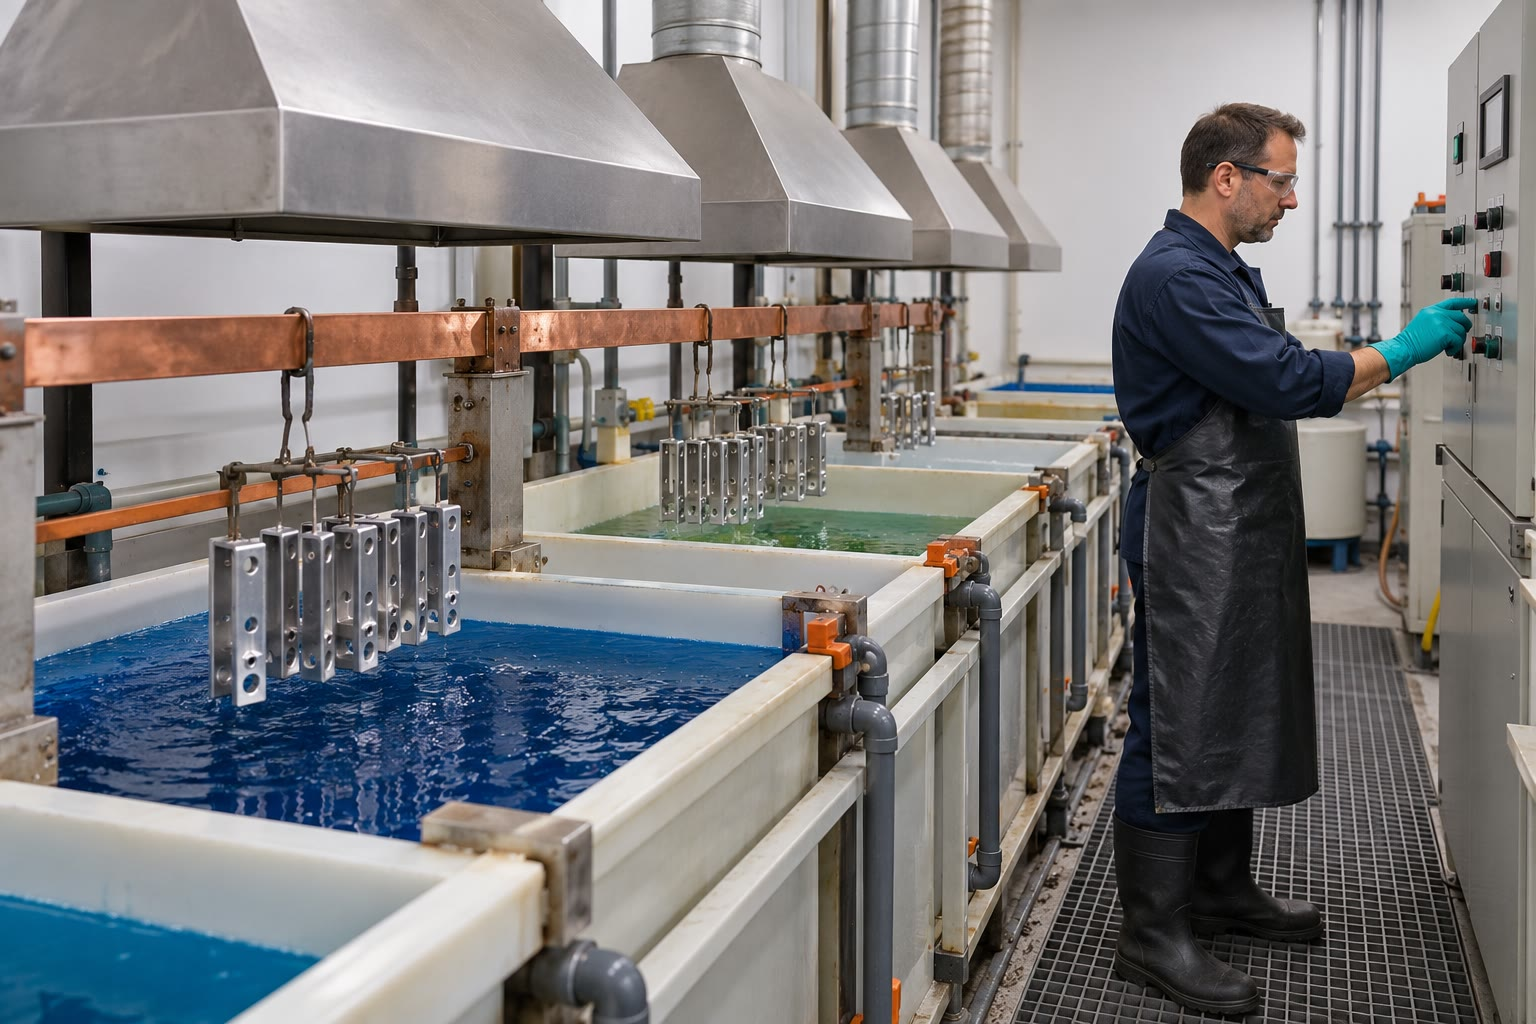
\includegraphics[width=0.62\linewidth]{images/book3/ai/b2-10-electroplating.jpg}

{\small Een galvaniseerlijn: de te bekleden onderdelen hangen aan koperen
stroomrails in de baden en worden als kathode geschakeld; de operator stelt de stroom
in aan de gelijkrichter. De stroom legt vast hoe snel metaal wordt afgezet; de potentiaal
van de onderdelen beslist welk metaal, of hoeveel waterstof, er samen mee ontstaat.}
\end{omfigure}

\section{Een elektrode buiten evenwicht}

\begin{definition}[Stroom-potentiaalkromme]\label{def:b2:current-potential-curves:ie-curve}
De \emph{stroom-potentiaalkromme}\index{stroom-potentiaalkromme} van een
elektrode in een oplossing is de grafiek van de stroom $i$ door de elektrode
als functie van haar potentiaal $E$. Een \emph{anodische stroom}\index{anodische stroom},
positief geteld, komt overeen met een oxidatie aan de elektrode; een
\emph{kathodische stroom}\index{kathodische stroom}, negatief geteld, met een
reductie.
\end{definition}

\begin{definition}[Elektroactief deeltje]\label{def:b2:current-potential-curves:electroactive}
Een \emph{elektroactief deeltje}\index{elektroactief deeltje} is een deeltje
dat aan de elektrode geoxideerd of gereduceerd kan worden in het beschouwde
potentiaalgebied.
\end{definition}

\begin{proposition}[Stroom en snelheid]\label{prop:b2:current-potential-curves:current-rate}
Als er aan een elektrode één enkele halfreactie met $n$ elektronen plaatsvindt, meet de
stroom haar snelheid: $i = nF\,d\xi/dt$, met $\xi$ de voortgang van
de oxidatie (zodat $i > 0$ voor een oxidatie, $i < 0$ voor een reductie).
\end{proposition}

\begin{proof}
Volgens \cref{prop:b2:cell-thermodynamics:charge} verplaatst een voortgang $d\xi$ de
lading $nF\,d\xi$ door de elektrode in de tijd $dt$.
\end{proof}

Om zo'n kromme op te nemen, moet de potentiaal van één elektrode opgelegd en
gemeten worden terwijl er een stroom door loopt --- wat een cel met twee elektroden
niet kan, omdat de stroom ook de potentiaal van de tweede
elektrode verandert.

\begin{definition}[Opstelling met drie elektroden]\label{def:b2:current-potential-curves:set-up}
In een opstelling met drie elektroden loopt de stroom tussen de
\emph{werkelektrode}\index{werkelektrode}, de bestudeerde elektrode, en de \emph{tegenelektrode}\index{tegenelektrode}, die de keten sluit; de potentiaal
van de werkelektrode wordt gemeten tegen een referentie-elektrode waardoor
geen stroom loopt. Een elektronische potentiostaat regelt de stroom zo
dat deze potentiaal de opgelegde waarde behoudt.
\end{definition}

\begin{omfigure}
\begin{tikzpicture}[font=\small, >={Stealth}]
  \pic[transform shape] at (0,0) {beaker={0.7}{omDef!14}};
  \pic at (-0.55,0.25) {electrode={black!35}};
  \pic at (0.55,0.25) {electrode={black!15}};
  \pic (r) at (0.0,0.15) {probe};
  \draw[thick, rounded corners] (-2.2,4.3) rectangle (2.2,5.5);
  \node at (0,4.9) {potentiostat};
  \draw[thick, omThm] (-0.40,2.65) -- (-0.40,3.5) -- (-1.6,3.5) -- (-1.6,4.3);
  \draw[thick, omDef] (0.70,2.65) -- (0.70,3.5) -- (1.6,3.5) -- (1.6,4.3);
  \draw[thick] (r-top) -- (0,4.3);
  \node[anchor=east, font=\scriptsize, omThm] at (-1.65,3.85) {WE};
  \node[anchor=west, font=\scriptsize, omDef] at (1.65,3.85) {TE};
  \node[anchor=west, font=\scriptsize] at (0.05,3.95) {RE};
  \draw[<-, omProp, thick] (-0.75,1.2) -- (-2.0,1.4) node[left, text=black, align=right] {werk-\\ elektrode};
  \draw[<-, omProp, thick] (0.85,1.2) -- (2.1,1.4) node[right, text=black, align=left] {tegen-\\ elektrode};
  \draw[<-, omProp, thick] (0.05,0.5) -- (1.4,-0.4) node[right, text=black] {referentie-elektrode};
  \node[font=\scriptsize, align=center] at (0,6.0) {legt $E_{\text{WE}} - E_{\text{RE}}$ op, meet $i$};
\end{tikzpicture}

{\small De opstelling met drie elektroden. De potentiostaat stuurt de stroom
tussen de \omterm{def:b2:current-potential-curves:set-up}{werkelektrode} (WE) en de \omterm{def:b2:current-potential-curves:set-up}{tegenelektrode} (TE) zo dat de potentiaal van de
\omterm{def:b2:current-potential-curves:set-up}{werkelektrode}, gemeten tegen de referentie-elektrode (RE), op de opgelegde waarde
blijft; door de referentie loopt geen stroom.}
\end{omfigure}

Wanneer er geen stroom loopt en beide vormen van een koppel aanwezig zijn, neemt de elektrode
de nernstpotentiaal van het koppel aan --- als de elektronenuitwisseling snel
genoeg is om die in te stellen. De potentiaal ervan weg bewegen laat een stroom
lopen.

\section{Snelle en trage systemen}

\begin{definition}[Overspanning]\label{def:b2:current-potential-curves:overpotential}
De \emph{overspanning}\index{overspanning} van een elektrode waardoor een
stroom $i$ loopt, is $\eta = E(i) - E_{\text{eq}}$, het verschil tussen haar
potentiaal en de evenwichtspotentiaal (van Nernst) van het koppel. De
\emph{drempelpotentiaal}\index{drempelpotentiaal} van een halfreactie is de
potentiaal waarboven haar stroom merkbaar wordt.
\end{definition}

\begin{definition}[Snelle en trage systemen]\label{def:b2:current-potential-curves:fast-slow}
Een koppel is een \emph{snel systeem}\index{snel systeem} aan een gegeven elektrode als er een
merkbare stroom loopt zodra de potentiaal van zijn nernstpotentiaal afwijkt;
het is een \emph{traag systeem}\index{traag systeem} als er een \omterm{def:b2:current-potential-curves:overpotential}{overspanning} van
enkele tienden volt nodig is voordat de stroom merkbaar wordt, in
beide richtingen.
\end{definition}

Of een systeem snel of traag is, hangt af van het koppel en van het
elektrodemateriaal. De koppels \ce{Fe^3+}/\ce{Fe^2+} en \ce{Ag+}/\ce{Ag} zijn snel op
platina; de reductie van \ce{H+} is snel op platina maar traag op kwik,
lood of zink; de oxidatie van water tot dizuurstof is traag op elke elektrode.
Elektronenoverdrachten die bindingen verbreken of vormen, zoals die van \ce{O2} of \ce{H2},
zijn doorgaans traag; de overdracht van een elektron tussen twee ionen van bijna
dezelfde vorm is snel. De vorm van het stijgende deel van een trage kromme komt van
de kinetiek van de elektronenoverdracht, die in het deel van jaar~3 wordt afgeleid.

\begin{omfigure}
\begin{tikzpicture}
\begin{axis}[omie, width=0.47\linewidth, height=5.4cm, xmin=0.25, xmax=1.3,
  ymin=-1.3, ymax=1.3, xlabel={$E$}, ylabel={$i$}, title={\small snel systeem}]
\addplot[omanodic] table[x=E, y=i, restrict expr to domain={\thisrow{i}}{0:2}] {figdata/out/bachelor-2-ie-curves-a.dat};
\addplot[omcathodic] table[x=E, y=i, restrict expr to domain={\thisrow{i}}{-2:0}] {figdata/out/bachelor-2-ie-curves-a.dat};
\draw[densely dotted] (axis cs:0.77,-1.2) -- (axis cs:0.77,1.2);
\node[font=\scriptsize, anchor=north west] at (axis cs:0.78,-0.05) {$E_{\text{eq}}$};
\node[font=\scriptsize, anchor=south] at (axis cs:1.1,1.0) {\ce{Fe^2+} $\to$ \ce{Fe^3+}};
\node[font=\scriptsize, anchor=north] at (axis cs:0.45,-1.0) {\ce{Fe^3+} $\to$ \ce{Fe^2+}};
\end{axis}
\end{tikzpicture}\hfill
\begin{tikzpicture}
\begin{axis}[omie, width=0.47\linewidth, height=5.4cm, xmin=-0.25, xmax=1.8,
  ymin=-1.3, ymax=1.3, xlabel={$E$}, ylabel={$i$}, title={\small traag systeem}]
\addplot[omanodic] table[x=E, y=i, restrict expr to domain={\thisrow{i}}{0:2}] {figdata/out/bachelor-2-ie-curves-c.dat};
\addplot[omcathodic] table[x=E, y=i, restrict expr to domain={\thisrow{i}}{-2:0}] {figdata/out/bachelor-2-ie-curves-c.dat};
\draw[densely dotted] (axis cs:0.77,-1.2) -- (axis cs:0.77,1.2);
\draw[<->, omProp] (axis cs:0.77,0.5) -- (axis cs:1.12,0.5) node[midway, above, font=\scriptsize] {$\eta_a$};
\draw[<->, omProp] (axis cs:0.42,-0.5) -- (axis cs:0.77,-0.5) node[midway, below, font=\scriptsize] {$\eta_c$};
\node[font=\scriptsize, anchor=north west] at (axis cs:0.78,-0.05) {$E_{\text{eq}}$};
\end{axis}
\end{tikzpicture}

{\small Modelkrommen stroom-potentiaal van een koppel waarvan de twee vormen
in gelijke concentraties aanwezig zijn (anodische tak rood, kathodische blauw). Links een \omterm{def:b2:current-potential-curves:fast-slow}{snel
systeem}: de stroom verandert steil van teken bij de evenwichtspotentiaal. Rechts
een \omterm{def:b2:current-potential-curves:fast-slow}{traag systeem}: over een potentiaalgebied eromheen loopt geen stroom; elke
tak vereist een \omterm{def:b2:current-potential-curves:overpotential}{overspanning}. Beide bereiken dezelfde grensplateaus, bepaald door
diffusie. (Illustratieve waarden.)}
\end{omfigure}

\section{Massatransport en grensstromen}

Wanneer de elektronenoverdracht snel is, wordt de stroom begrensd door de aanvoer van
de beginstof naar de elektrode. In een geroerde oplossing blijft een dunne vloeistoflaag
tegen de elektrode bijna stil, en de beginstof steekt die over door
diffusie.

\begin{definition}[Diffusielaag en grensstroom]\label{def:b2:current-potential-curves:limiting-current}
De \emph{diffusielaag}\index{diffusielaag} is de laag oplossing,
met dikte $\delta$ (enkele tot tientallen micrometers in een geroerde
oplossing), tegen de elektrode, waarin deeltjes zich alleen door diffusie
verplaatsen. De \emph{grensstroom}\index{grensstroom} is de stroom
die bereikt wordt wanneer het \omterm{def:b2:current-potential-curves:electroactive}{elektroactieve deeltje} even snel verbruikt wordt als het aankomt,
zodat zijn concentratie aan het oppervlak nul is.
\end{definition}

\begin{omfigure}
\begin{tikzpicture}[font=\small, >={Stealth}, x=1.2cm, y=1.2cm]
  \fill[black!25] (-0.4,0) rectangle (0,3);
  \node[rotate=90, font=\scriptsize] at (-0.2,1.5) {elektrode};
  \draw[->] (0,0) -- (4.6,0) node[right] {$x$};
  \draw[->] (0,0) -- (0,3.2) node[above] {$c$};
  \draw[densely dashed] (1.6,0) -- (1.6,3);
  \node[below, font=\scriptsize] at (1.6,0) {$\delta$};
  \draw[omDef, thick] (0,1.2) -- (1.6,2.4) -- (4.4,2.4);
  \draw[omThm, thick] (0,0.02) -- (1.6,2.4);
  \node[font=\scriptsize, anchor=west] at (2.6,2.6) {bulk, $c^b$ (geroerd)};
  \node[font=\scriptsize, omDef, anchor=east] at (-0.45,1.2) {$c^s$};
  \node[font=\scriptsize, omThm, anchor=west] at (1.7,0.5) {$c^s = 0$: grensstroom};
  \node[font=\scriptsize, align=center] at (0.8,3.0) {diffusie-\\ laag};
\end{tikzpicture}

{\small Concentratie van de beginstof bij een elektrode in een geroerde
oplossing. Over de \omterm{def:b2:current-potential-curves:limiting-current}{diffusielaag} is het profiel lineair; de flux, en dus de
stroom, is evenredig met $c^b - c^s$. Hij is het grootst wanneer de beginstof
verbruikt wordt zodra hij aankomt ($c^s = 0$, rood).}
\end{omfigure}

\begin{theorem}[Grensstroom]\label{thm:b2:current-potential-curves:limiting}
Voor een deeltje met bulkconcentratie $c$ en diffusiecoëfficiënt $D$,
dat een \omterm{def:b2:current-potential-curves:limiting-current}{diffusielaag} met dikte $\delta$ oversteekt naar een elektrode met oppervlakte $A$,
is de \omterm{def:b2:current-potential-curves:limiting-current}{grensstroom}, in absolute waarde,
\[
  |i_{\lim}| = \frac{nFADc}{\delta} .
\]
\end{theorem}

\begin{proof}
In stationaire toestand is het concentratieprofiel in de laag lineair (de tweede wet van
Fick met $\partial c/\partial t = 0$ geeft $d^2c/dx^2 = 0$), dus de flux
naar de elektrode is $j = D(c - c^s)/\delta$, in mol per eenheid oppervlakte en
tijd. Elk molecuul dat aankomt, reageert met $n$ elektronen: $|i| = nFAj =
nFAD(c - c^s)/\delta$, het grootst voor $c^s = 0$.
\end{proof}

\begin{example}[Grootte van een grensstroom]\label{ex:b2:current-potential-curves:ilim}
Voor een deeltje bij \qty{10}{mmol/L} (\qty{10}{mol/m^3}), met $D =
\qty{7e-10}{m^2/s}$, $\delta = \qty{20}{\micro m}$, $n = 1$, op
\qty{1.0}{cm^2} is $|i_{\lim}| = 96\,485 \times 10^{-4} \times 7 \times 10^{-10}
\times 10/(2 \times 10^{-5}) = \qty{3.4}{mA}$.
\end{example}

\begin{theorem}[Golf van een snel systeem]\label{thm:b2:current-potential-curves:wave}
Voor een snel koppel $\mathrm{Ox} + n\,\mathrm e^- \rightleftharpoons \mathrm{Red}$,
met anodische \omterm{def:b2:current-potential-curves:limiting-current}{grensstroom} $i_{\lim,a} > 0$ (bepaald door Red) en kathodische
\omterm{def:b2:current-potential-curves:limiting-current}{grensstroom} $i_{\lim,c} < 0$ (bepaald door Ox), is de stationaire kromme
\[
  E = E_{1/2} + \frac{RT}{nF}\ln\frac{i - i_{\lim,c}}{i_{\lim,a} - i},
  \qquad E_{1/2} = E^\circ + \frac{RT}{nF}\ln\frac{D_{\text{Red}}}{D_{\text{Ox}}} ,
\]
waarbij de laagdikte voor beide vormen dezelfde is.
\end{theorem}

\begin{proof}
\omterm{def:b2:current-potential-curves:fast-slow}{Snel systeem}: aan het oppervlak geldt Nernst: $E = E^\circ + (RT/nF)
\ln(c^s_{\text{Ox}}/c^s_{\text{Red}})$. Lineaire profielen: een \omterm{def:b2:current-potential-curves:ie-curve}{anodische stroom} $i$
verbruikt Red en produceert Ox aan het oppervlak, $i = nFAD_{\text{Red}}(c^b_{\text{Red}}
- c^s_{\text{Red}})/\delta = -nFAD_{\text{Ox}}(c^b_{\text{Ox}} - c^s_{\text{Ox}})/\delta$.
Met $i_{\lim,a} = nFAD_{\text{Red}}c^b_{\text{Red}}/\delta$ en $i_{\lim,c} =
-nFAD_{\text{Ox}}c^b_{\text{Ox}}/\delta$ geven die $c^s_{\text{Red}} = (i_{\lim,a} -
i)\delta/(nFAD_{\text{Red}})$ en $c^s_{\text{Ox}} = (i - i_{\lim,c})\delta/(nFAD_{\text{Ox}})$.
Substitueer dit in de vergelijking van Nernst.
\end{proof}

\begin{corollary}[Halvegolfpotentiaal]\label{cor:b2:current-potential-curves:half-wave}
Wanneer de twee vormen gelijke diffusiecoëfficiënten hebben, is $E_{1/2} = E^\circ$: met
slechts één vorm aanwezig is de stroom bij de standaardpotentiaal van het koppel
de helft van zijn grenswaarde.
\end{corollary}

\begin{proof}
Met alleen Red aanwezig is $i_{\lim,c} = 0$, en voor $i = i_{\lim,a}/2$ verdwijnt de logaritme:
$E = E_{1/2} = E^\circ$ wanneer $D_{\text{Red}} = D_{\text{Ox}}$.
\end{proof}

\begin{proposition}[Plateaus meten concentraties]\label{prop:b2:current-potential-curves:plateau}
Bij vaste roering en elektrode is de hoogte van een plateau evenredig met de
concentratie van het deeltje dat het verbruikt: een elektrode die op een
potentiaal op het plateau gehouden wordt, is een amperometrische sensor.
\end{proposition}

\begin{proof}
$|i_{\lim}| = (nFAD/\delta)\,c$ en de factor tussen haakjes is constant bij vaste
roering en temperatuur.
\end{proof}

\begin{omfigure}
\begin{tikzpicture}
\begin{axis}[omie, width=0.47\linewidth, height=5.0cm, xmin=0.25, xmax=1.3,
  ymin=-0.3, ymax=1.3, xlabel={$E$}, ylabel={$i$}, title={\small alleen \ce{Fe^2+} aanwezig}]
\addplot[omanodic] table[x=E, y=i] {figdata/out/bachelor-2-ie-curves-b.dat};
\draw[densely dotted] (axis cs:0.77,0) -- (axis cs:0.77,0.5) -- (axis cs:0.25,0.5);
\node[font=\scriptsize, anchor=north] at (axis cs:0.77,-0.02) {$E_{1/2}$};
\node[font=\scriptsize, anchor=south west] at (axis cs:0.27,0.5) {$i_{\lim}/2$};
\node[font=\scriptsize, anchor=south] at (axis cs:1.12,1.0) {plateau};
\end{axis}
\end{tikzpicture}\hfill
\begin{tikzpicture}
\begin{axis}[width=0.42\linewidth, height=5.0cm, xmin=0, xmax=1.05, ymin=0, ymax=1.1,
  axis x line=bottom, axis y line=left, xtick=\empty, ytick=\empty,
  xlabel={$c$}, ylabel={$i_{\lim}$}, label style={font=\small},
  title={\small amperometrie}]
\addplot[omanodic, mark=*, mark size=1.2pt] table[x=c, y=i] {figdata/out/bachelor-2-ie-curves-e.dat};
\end{axis}
\end{tikzpicture}

{\small Links: de golf van een snel koppel wanneer alleen de gereduceerde vorm aanwezig is
(model); de halve hoogte ligt bij de halvegolfpotentiaal. Rechts: de plateauhoogte
groeit evenredig met de concentratie.}
\end{omfigure}

\section{Het oplosmiddel en de elektrode}

Water is zelf elektroactief: het wordt geoxideerd tot dizuurstof
(\ce{2H2O -> O2 + 4H+ + 4e-}) en gereduceerd tot diwaterstof (\ce{2H+ + 2e- -> H2}, of
\ce{2H2O + 2e- -> H2 + 2OH-}). Omdat het oplosmiddel nooit uitgeput raakt, hebben zijn krommen
geen plateau: ze stijgen steil en begrenzen elke andere kromme.

\begin{definition}[Elektroactiviteitsvenster]\label{def:b2:current-potential-curves:window}
De \emph{oplosmiddelmuren}\index{oplosmiddelmuur} zijn de steile takken van de
oxidatie en de reductie van het oplosmiddel. Het
\emph{elektroactiviteitsvenster}\index{elektroactiviteitsvenster} is het potentiaalgebied
ertussen, waarin de krommen van de opgeloste deeltjes waargenomen kunnen worden.
\end{definition}

\begin{proposition}[Het venster van water]\label{prop:b2:current-potential-curves:window}
In water bij een gegeven pH ligt het venster rond het thermodynamische gebied van de
twee koppels van water, $\qty{0}{V} - 0.059\,\mathrm{pH}$ en $\qty{1.23}{V} -
0.059\,\mathrm{pH}$, aan elke kant verbreed met de \omterm{def:b2:current-potential-curves:overpotential}{overspanning} van de
overeenkomstige reactie op de gebruikte elektrode.
\end{proposition}

\begin{proof}[Redenering]
Elke muur begint dicht bij de nernstpotentiaal van zijn koppel, verschoven met de
drempeloverspanning: de oxidatie van water is traag op alle elektroden, dus
de anodische muur ligt enkele tienden volt boven \qty{1.23}{V} (bij pH 0); de
reductie van \ce{H+} is snel op platina, waarvan de kathodische muur dicht bij
\qty{0}{V} blijft, maar traag op zink, lood of kwik, waarvan de muur enkele tienden
volt lager ligt.
\end{proof}

\begin{omfigure}
\begin{tikzpicture}
\begin{axis}[omie, width=0.82\linewidth, height=5.4cm, xmin=-1.2, xmax=2.0,
  ymin=-3, ymax=3, xlabel={$E$ (V)}, ylabel={$i$}, clip=true, clip mode=individual]
\addplot[omwall] table[x=E, y=i] {figdata/out/bachelor-2-ie-curves-d-high.dat};
\addplot[omcathodic] table[x=E, y=i, restrict expr to domain={\thisrow{E}}{-1.2:0.6}] {figdata/out/bachelor-2-ie-curves-d-Pt.dat};
\addplot[omanodic] table[x=E, y=i, restrict expr to domain={\thisrow{E}}{0.6:2.0}] {figdata/out/bachelor-2-ie-curves-d-Pt.dat};
\draw[densely dotted] (axis cs:0,-2.8) -- (axis cs:0,2.8);
\draw[densely dotted] (axis cs:1.23,-2.8) -- (axis cs:1.23,2.8);
\node[font=\scriptsize, anchor=north west] at (axis cs:0.02,-0.1) {0};
\node[font=\scriptsize, anchor=north west] at (axis cs:1.24,-0.1) {1.23};
\node[font=\scriptsize, omDef, anchor=west] at (axis cs:0.05,-2.2) {\ce{H+} $\to$ \ce{H2} op Pt};
\node[font=\scriptsize, gray, anchor=east] at (axis cs:-0.85,-1.0) {op Zn, Pb};
\node[font=\scriptsize, omThm, anchor=east] at (axis cs:1.18,2.2) {\ce{H2O} $\to$ \ce{O2}};
\end{axis}
\end{tikzpicture}

{\small De muren van water bij pH 0 (model). De reductie van \ce{H+} begint rond
\qty{0}{V} op platina (blauw), maar enkele tienden volt lager op metalen zoals
zink of lood (gestreept); de oxidatie van water vereist op elke
elektrode een \omterm{def:b2:current-potential-curves:overpotential}{overspanning}. Het venster is het gebied tussen de muren.}
\end{omfigure}

\section{Krommen lezen}

\begin{method}[De krommen van een oplossing schetsen]\label{met:b2:current-potential-curves:sketch-ie}
\begin{enumerate}
  \item Teken de twee muren van het oplosmiddel voor de pH en het
        elektrodemateriaal.
  \item Plaats voor elk aanwezig koppel zijn nernstpotentiaal (beide vormen
        aanwezig) of $E^\circ$ (één vorm): een \omterm{def:b2:current-potential-curves:fast-slow}{snel systeem} snijdt de as daar
        steil; een \omterm{def:b2:current-potential-curves:fast-slow}{traag systeem} is verschoven met zijn \omterm{def:b2:current-potential-curves:overpotential}{overspanningen}.
  \item Geef elke golf een plateau evenredig met de concentratie van het
        deeltje dat ze verbruikt; een metalen elektrode die zichzelf oxideert, heeft geen
        plateau (het metaal raakt niet uitgeput).
  \item Tel de stromen op van de reacties die bij elke potentiaal mogelijk zijn.
\end{enumerate}
\end{method}

\begin{method}[De krommen lezen]\label{met:b2:current-potential-curves:read-ie}
\begin{enumerate}
  \item Lees bij een opgelegde potentiaal op elke kromme de stroom van elke
        reactie af: ze verlopen gelijktijdig, in verhouding tot hun stromen.
  \item Zoek bij een opgelegde stroom (elektrolyse) de potentiaal waarbij de
        anodische of kathodische krommen samen die stroom geven; de betrokken reacties
        zijn die waarvan de krommen daar bijdragen.
  \item Voor een cel, of een corroderend metaal, is de \omterm{def:b2:current-potential-curves:ie-curve}{anodische stroom} van de ene reactie
        gelijk aan de \omterm{def:b2:current-potential-curves:ie-curve}{kathodische stroom} van de andere: zoek dat paar
        punten.
\end{enumerate}
\end{method}

\begin{example}[Verzinken vanuit een zuur bad]\label{ex:b2:current-potential-curves:zinc}
In een zuur zinkbad heeft de kathode twee mogelijke reducties: \ce{Zn^2+
+ 2e- -> Zn} ($E^\circ = \qty{-0.76}{V}$, snel) en \ce{2H+ + 2e- -> H2}
($E^\circ = \qty{0}{V}$). Thermodynamisch zou eerst waterstof moeten ontstaan, en zink
nooit. Maar op zink is de reductie van \ce{H+} traag: haar muur ligt onder
\qty{-0.76}{V}, en bij de potentiaal waarbij zink met een bruikbare snelheid
wordt afgezet, ontstaat er weinig waterstof. De kromme, niet het diagram, verklaart het
verzinken.
\end{example}

\begin{history}[Polarografie]
\begin{minipage}[t]{0.25\linewidth}
\vspace{0pt}
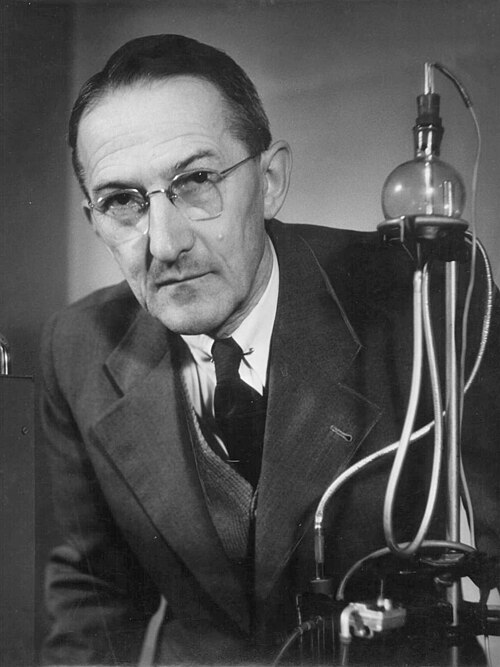
\includegraphics[width=\linewidth]{images/book3/heyrovsky.jpg}
\end{minipage}\hfill
\begin{minipage}[t]{0.71\linewidth}
\vspace{0pt}
In 1922 nam Jaroslav Heyrovský de stroom op door een kwikelektrode die
druppel na druppel ontstond aan het uiteinde van een capillair, terwijl de potentiaal werd
gevarieerd: elk reduceerbaar deeltje gaf een trap waarvan de positie het identificeerde en
waarvan de hoogte zijn concentratie mat. De vernieuwde druppel hield het oppervlak
vers, en de hoge \omterm{def:b2:current-potential-curves:overpotential}{overspanning} van waterstof op kwik opende een breed
kathodisch venster. De polarografie leverde hem in 1959 de Nobelprijs voor Scheikunde op
en legde de grondslag van de elektroanalytische chemie; de foto toont hem met een
druppelende kwikelektrode. (Foto: archief van het J.~Heyrovský-instituut
voor fysische chemie, CC BY-SA 3.0, Wikimedia Commons.)
\end{minipage}
\end{history}

\section{Oefeningen}

\begin{exercise}[$\star$]\label{exo:b2:current-potential-curves:1}
Geef in een daniellcel die een stroom levert, het teken van de stroom aan de
zinkelektrode en aan de koperelektrode, met de afspraken van dit
hoofdstuk.
\end{exercise}

\begin{exercise}[$\star$]\label{exo:b2:current-potential-curves:2}
Bereken de \omterm{def:b2:current-potential-curves:limiting-current}{grensstroom} van de reductie van \ce{Ag+} (\qty{2.0}{mmol/L}, $D =
\qty{1.6e-9}{m^2/s}$) op \qty{0.50}{cm^2} met $\delta = \qty{25}{\micro m}$
(modelwaarden).
\end{exercise}

\begin{exercise}[$\star$]\label{exo:b2:current-potential-curves:3}
Hoe herken je op de modelkrommen van het hoofdstuk een snel en een \omterm{def:b2:current-potential-curves:fast-slow}{traag
systeem}? Geef van elk een voorbeeld op platina.
\end{exercise}

\begin{exercise}[$\star$]\label{exo:b2:current-potential-curves:4}
Een oplossing bevat alleen \ce{Fe^2+}. Bij welke potentiaal bereikt haar \omterm{def:b2:current-potential-curves:ie-curve}{anodische stroom}
de helft van haar plateau, als de twee vormen even snel diffunderen ($E^\circ = \qty{0.77}{V}$)?
\end{exercise}

\begin{exercise}[$\star\star$]\label{exo:b2:current-potential-curves:5}
Een platina-elektrode in een oplossing van \ce{Fe^3+} en \ce{Cu^2+} (gelijke
concentraties, $E^\circ$ = 0.77 en \qty{0.34}{V}) wordt naar negatieve
potentialen gevarieerd. Beschrijf de kromme: golven, plateaus, hun hoogten, en de
kathodische muur.
\end{exercise}

\begin{exercise}[$\star\star$]\label{exo:b2:current-potential-curves:6}
In de oplossing van \cref{exo:b2:current-potential-curves:5} wordt de potentiaal van
de elektrode op \qty{0.50}{V} gehouden, en daarna op \qty{0.10}{V}. Wat gebeurt er in
elk geval?
\end{exercise}

\begin{exercise}[$\star\star$]\label{exo:b2:current-potential-curves:7}
Geef de nernstpotentialen van de twee koppels van water bij pH 0 en pH 14, en
schets hoe het venster op platina met de pH verschuift.
\end{exercise}

\begin{exercise}[$\star\star$]\label{exo:b2:current-potential-curves:8}
\ce{Fe^2+} wordt getitreerd met \ce{Ce^4+} terwijl een platina-elektrode die op
\qty{1.0}{V} gehouden wordt, de stroom registreert. Schets de stroom als functie van het toegevoegde volume
en leg uit hoe hij de equivalentie lokaliseert (\ce{Ce^4+}/\ce{Ce^3+}: $E^\circ =
\qty{1.72}{V}$).
\end{exercise}

\begin{exercise}[$\star\star$]\label{exo:b2:current-potential-curves:9}
Een verdubbeling van de roersnelheid halveert de dikte van de \omterm{def:b2:current-potential-curves:limiting-current}{diffusielaag}. Wat
gebeurt er met de plateaus, de halvegolfpotentiaal en de nulstroompotentiaal
van een \omterm{def:b2:current-potential-curves:fast-slow}{snel systeem}?
\end{exercise}

\begin{exercise}[$\star\star\star$]\label{exo:b2:current-potential-curves:10}
Leid de vergelijking af van de golf van een \omterm{def:b2:current-potential-curves:fast-slow}{snel systeem} met alleen Red aanwezig, en
toon aan dat een grafiek van $E$ tegen $\log[i/(i_{\lim} - i)]$ een rechte is met
helling $0.059/n$ volt bij \qty{25}{\degreeCelsius}.
\end{exercise}

\begin{exercise}[$\star\star\star$]\label{exo:b2:current-potential-curves:11}
Een stuk zink dat in zuur van \qty{1}{mol/L} gedompeld wordt, lost slechts langzaam op, terwijl
hetzelfde stuk dat een platinadraad raakt, snel oplost, met waterstofbellen
op het platina. Verklaar met \omterm{def:b2:current-potential-curves:ie-curve}{stroom-potentiaalkrommen}.
\end{exercise}

\begin{exercise}[$\star\star\star$]\label{exo:b2:current-potential-curves:12}
Zou je, om een deeltje te oxideren waarvan de golf bij pH 0 op \qty{2.0}{V} ligt, een
platina-elektrode kiezen of een met een hoge zuurstofoverspanning? Leg uit, en zeg
wat er anders zou ontstaan.
\end{exercise}

\section{Probleem: een zuurstofsonde voor een rivier}

\begin{problem}[{Weekendprobleem --- de kathode van een amperometrische
zuurstofsensor, de grensstroom door zijn membraan, de ijking in
met lucht verzadigd water met de wet van Henry, en het zuurstofgehalte van een rivier}]
\label{pb:b2:current-potential-curves:1}
Een amperometrische zuurstofsonde heeft een gouden kathode en een zilveren anode in een
kaliumchloridegel, van het monster gescheiden door een dun, gasdoorlatend
membraan. De kathode wordt op \qty{-0.60}{V} gehouden tegen de zilver-zilverchloride-anode.
Gegevens bij \qty{25}{\degreeCelsius}: \omterm{prop:b2:chemical-potential:henry}{henryconstante} van
\ce{O2}, $H = \qty{1.3e-5}{mol/(m^3.Pa)}$; dampdruk van water
\qty{3.17}{kPa}; zuurstof in droge lucht 20.95~\% in volume; $E^\circ(\ce{O2}/\ce{H2O}) =
\qty{1.229}{V}$; $E^\circ(\ce{AgCl}/\ce{Ag}) = \qty{0.222}{V}$. Membraan (modelwaarden):
oppervlakte \qty{0.10}{cm^2}, dikte \qty{25}{\micro m}, effectieve
diffusiecoëfficiënt van \ce{O2} erdoorheen \qty{1.0e-10}{m^2/s}.
% ledger: henry:O2, pvap:H2O.298, air:O2, dfg:Cl-_ao, dfg:AgCl_cr, aw:O

\medskip
\noindent\textbf{Deel I --- De kathode.}
\begin{enumerate}
  \item Schrijf de reductie van dizuurstof in neutraal milieu op.
  \item Schrijf de reactie aan de zilveranode op, en de totale reactie.
  \item Bereken de nernstpotentiaal van het koppel \ce{O2}/\ce{H2O} bij pH 7 met
        $p_{\ce{O2}} = \qty{0.21}{bar}$.
  \item Druk de kathodepotentiaal, \qty{-0.60}{V} tegen Ag/AgCl, uit op de
        waterstofschaal, met de chloride-activiteit van de gel gelijk aan 1.
  \item Waarom moet de kathode ver onder de nernstpotentiaal van
        \ce{O2} gehouden worden?
  \item Waarom wordt een potentiaal op het plateau gekozen?
  \item Wat bepaalt de ondergrens van de bruikbare potentialen?
\end{enumerate}

\medskip
\noindent\textbf{Part II --- The limiting current.}
\noindent\textbf{Deel II --- De \omterm{def:b2:current-potential-curves:limiting-current}{grensstroom}.}
\begin{enumerate}[resume]
  \item Beschrijf het concentratieprofiel van \ce{O2} over het membraan wanneer de
        kathode op haar plateau werkt.
  \item Schrijf de flux van \ce{O2} door het membraan op.
  \item Leid de stroom af als functie van de concentratie $c$ van opgeloste
        \ce{O2}.
  \item Waarom wordt de membraandikte gebruikt in plaats van de \omterm{def:b2:current-potential-curves:limiting-current}{diffusielaag}?
  \item Waarom hangt de meting weinig af van de stroming van de rivier, maar
        sterk van vervuiling van het membraan?
\end{enumerate}

\medskip
\noindent\textbf{Deel III --- IJking.}
\begin{enumerate}[resume]
  \item Bereken de partiële druk van \ce{O2} boven water dat met lucht verzadigd is bij
        \qty{1.013}{bar} en \qty{25}{\degreeCelsius}.
  \item Bereken de concentratie opgeloste \ce{O2} bij verzadiging, in
        \unit{mol/m^3}.
  \item Druk ze uit in \unit{mg/L}.
  \item Voorspel de stroom van de sonde in met lucht verzadigd water.
  \item De sonde leest in met lucht verzadigd water in werkelijkheid \qty{4.05}{\micro A} af
        (gegevens voor de oefening). Bereken haar gevoeligheid in \unit{\micro A} per
        \unit{mg/L}.
  \item Waarom ijken in plaats van op de voorspelde stroom te vertrouwen?
  \item Wat zou de sonde moeten aangeven in water zonder zuurstof?
\end{enumerate}

\medskip
\noindent\textbf{Deel IV --- De rivier.}
\begin{enumerate}[resume]
  \item In een riviermonster bij \qty{25}{\degreeCelsius} geeft de sonde
        \qty{2.80}{\micro A} aan. Bereken de opgeloste zuurstof in \unit{mg/L}.
  \item Druk die uit als percentage van de verzadiging.
  \item Het water van een rivier is aan de bron bijna verzadigd met zuurstof.
        Stel een oorzaak voor het tekort voor.
  \item Welke hoeveelheid \ce{O2} verbruikt de sonde in één uur? Verstoort ze
        het monster?
  \item Waarom moet de ijking herhaald worden als de rivier \qty{15}{\degreeCelsius} heeft?
  \item Geef de concentratie opgeloste zuurstof van het monster.
\end{enumerate}
\end{problem}
